% Anonymous review manuscript for Cybernetics and Systems (Taylor & Francis).
% Compile with: pdflatex manuscript; bibtex manuscript; pdflatex manuscript; pdflatex manuscript.
\documentclass[11pt,a4paper]{article}
\usepackage[T1]{fontenc}
\usepackage[utf8]{inputenc}
\usepackage[margin=2.5cm]{geometry}
\usepackage{graphicx}
\usepackage{booktabs}
\usepackage{array}
\usepackage{amsmath}
\usepackage{caption}
\usepackage{float}
\usepackage{microtype}
\usepackage[hidelinks]{hyperref}
\usepackage{url}
\usepackage[numbers,sort&compress]{natbib}
\setlength{\parskip}{0.4em}
\setlength{\parindent}{0pt}

\title{How Far Do Explainable Detectors of Digital Deception Generalise?\\
A Cross-Dataset Evaluation of an Intelligent Multi-Module System}
\author{Anonymous authors}
\date{}

\begin{document}
\maketitle

\begin{abstract}
Digital deception detectors often report high in-domain accuracy, but deployment exposes them to changing generators, corpora, and organisations. We evaluate an explainable system for synthetic images, fake news, and recruitment fraud using cross-dataset tests, confidence intervals, significance tests, and grouped validation. Image accuracy falls from 95.4\% in-domain to approximately chance elsewhere; mixed-source training repairs transfer between known image sources but not to an independently collected set. News classifiers similarly fail on claim-level data, while recruitment F$_1$ falls from 0.85 to 0.60 for unseen employers. Model-derived explanations expose dataset-specific cues. Evaluation across environments is therefore essential for trustworthy practical intelligent systems.
\end{abstract}

\textbf{Keywords:} digital deception; explainable AI; cross-dataset evaluation; intelligent systems; domain shift

\textbf{Word count:} approximately 5,400 words (including tables and captions; excluding references)

\section{Introduction}
A synthetic profile photograph, a rewritten news story and a fabricated job advertisement exploit the same weakness: users cannot cheaply verify what they see. Research has progressed on each threat separately, with convolutional and transformer detectors for synthetic faces \cite{soudy2024deepfake,yan2023deepfakebench}, supervised models for fake news \cite{ahmed2017isot,verma2021welfake}, and a smaller literature on recruitment fraud \cite{naude2023recruitment,taneja2025fraudbert}. Two practical problems remain. First, accuracy is often reported on the corpus used for training, which hides how much a model has learned dataset-specific cues rather than the underlying phenomenon. Second, explanations shown to users are not always evaluated quantitatively, which limits their value as evidence \cite{tsigos2024quantitative}.

This paper evaluates a three-module pipeline with these problems in mind. Our contributions are:
\begin{enumerate}
\item A protocol that evaluates each detector in-domain and on different data, applied to synthetic face images, fake news and recruitment scams in one study, with confidence intervals, significance tests and repeated splits.
\item Image-classification results at two scales: four architectures and an ablation trained on 10{,}000 images, and a ResNet50-feature classifier trained on all 100{,}000 images of a 140{,}000-image face dataset (95.4\% test accuracy), followed by tests on two other image sets on which all five image models fail, and an experiment on whether mixing training sources repairs the failure.
\item A fake-news study on ISOT, WELFake and LIAR, with label-leaking source tags removed and duplicates dropped, that quantifies the generalisation gap, shows what the models learned and shows that pooling article corpora does not help on claim-level data.
\item A recruitment-scam classifier trained on EMSCAD, compared against the rule-based method of our earlier prototype, with a grouped-by-employer evaluation that separates generalisation to new employers from memorisation.
\item Explanations computed from the models (Grad-CAM; exact linear word contributions) and a quantitative measurement of where the image model attends.
\end{enumerate}
The study asks four research questions: \emph{RQ1}, how accurately do the detectors classify
held-out data from their training environments? \emph{RQ2}, how much performance is retained
under a change of image source, news corpus, or employer? \emph{RQ3}, does mixed-source training
repair image-domain shift? \emph{RQ4}, do model-derived explanations reveal plausible evidence or
dataset-specific shortcuts? We state the limits of the study plainly in Section~\ref{sec:limits}.

\section{Related Work}
\textbf{Synthetic-image and deepfake detection.} Convolutional networks and vision transformers
remain common detector families \cite{soudy2024deepfake,mirsky2021deepfakes}. However,
DeepfakeBench shows that preprocessing and evaluation choices impede fair comparison, while
cross-dataset studies report substantial deterioration on unseen manipulations
\cite{yan2023deepfakebench,nadimpalli2022crossdataset}. FaceForensics++ established a widely used
benchmark for manipulated facial imagery \cite{rossler2019faceforensics}, but performance on a
fixed benchmark does not by itself establish transfer to new generators. Synthetic-image detectors may also exploit
generator-specific artefacts \cite{wang2020cnngenerated}. Explainable detectors commonly use
Grad-CAM \cite{selvaraju2017gradcam,mansoor2025xai}, but quantitative evaluation of explanation
quality remains uncommon \cite{tsigos2024quantitative}; saliency-map sanity checks and
perturbation-based evaluation provide stronger tests of faithfulness
\cite{adebayo2018sanity,petsiuk2018rise}.

\textbf{Fake news.} Article-level corpora such as ISOT and WELFake support high in-domain scores
\cite{ahmed2017isot,verma2021welfake}, whereas LIAR contains short fact-checked claims with a
different label construction \cite{wang2017liar}. Recent cross-dataset analysis attributes
near-ceiling benchmark results partly to structural homogeneity and provenance cues
\cite{calvo2026generalization}. LIME and SHAP are widely used explanation frameworks
\cite{ribeiro2016lime,lundberg2017shap}, although a linear classifier permits exact additive term
contributions without a surrogate model.

\textbf{Recruitment fraud.} Public data are scarce; EMSCAD is the principal public corpus
\cite{vidros2017emscad}. Later work applies conventional machine learning and transformers
\cite{naude2023recruitment,taneja2025fraudbert}. Most evaluations randomly divide postings, so
records from related employers can occur in training and testing; our grouped protocol measures a
different and more demanding deployment condition.

\section{Materials and Data Preparation}
\label{sec:data}
\textbf{Face images.} We use a face dataset of 140{,}000 images: 100{,}000 for training, 20{,}000 for validation and 20{,}000 for testing, each split balanced between real and GAN-generated faces; the real images derive from Flickr-Faces-HQ \cite{karras2019stylegan}. Two further sets are used \emph{only for testing}: 3{,}000 images (1{,}500 per class) sampled from the CIFAKE test split \cite{bird2024cifake}, which contains real photographs and Stable-Diffusion-generated images at $32\times32$ resolution, and 999 images from a separate collection used in the project (436 real, 563 AI-generated, of mixed origin).

\textbf{Fake news.} ISOT \cite{ahmed2017isot} has 23{,}481 fake and 21{,}417 real articles; WELFake \cite{verma2021welfake} merges four corpora (72{,}134 articles); LIAR \cite{wang2017liar} has 12{,}836 PolitiFact statements with six truth labels, which we binarise (false, barely-true and pants-fire as fake). ISOT is known to be easy: in our copy 98.7\% of real articles contain ``(Reuters)'' in the first 120 characters and none of the fake ones do. For ISOT and WELFake we therefore remove Reuters datelines, URLs and image-credit boilerplate, drop texts shorter than 15 words, and remove exact duplicates (26\% of ISOT fake articles were duplicates), leaving 38{,}794 ISOT and 63{,}092 WELFake articles. WELFake's released labels are 1 = fake (37{,}106 rows) although its documentation states the opposite; we follow the row counts.

\textbf{Recruitment postings.} EMSCAD \cite{vidros2017emscad} contains 17{,}880 postings, 866 of them fraudulent. After removing exact duplicates, so that no posting appears in both training and test data, 15{,}879 remain (713 fraudulent, 4.5\%).

\textbf{Splits.} ISOT, WELFake and EMSCAD are split 70/15/15 with stratification (fixed seed); LIAR keeps its official split. Table~\ref{tab:data} lists the sizes.

\begin{table}[h]
\centering
\caption{Data used. Test sets are never used for training or model selection.}\label{tab:data}
\begin{tabular}{llrrr}
\toprule
Task & Dataset & Total & Train & Test \\
\midrule
Images & Face dataset (full-data run) & 140{,}000 & 100{,}000 & 20{,}000 \\
Images & Face dataset (subset runs) & 140{,}000 & 10{,}000 & 6{,}000 \\
Images & CIFAKE (test only) & -- & -- & 3{,}000 \\
Images & Local independently collected set (test only) & -- & -- & 999 \\
Fake news & ISOT (cleaned) & 38{,}794 & 27{,}155 & 5{,}820 \\
Fake news & WELFake (cleaned) & 63{,}092 & 44{,}164 & 9{,}464 \\
Fake news & LIAR (binary) & 12{,}836 & 10{,}269 & 1{,}283 \\
Recruitment & EMSCAD (deduplicated) & 15{,}879 & 11{,}115 & 2{,}382 (107 scams) \\
\bottomrule
\end{tabular}
\end{table}

\section{Methods}
\subsection{System architecture and decision support}
The system has three independent sensing modules rather than a single multimodal classifier. The
image module returns a real/synthetic label, score, and Grad-CAM map; the news module returns a
real/fake label, score, and signed term contributions; and the recruitment module returns a
legitimate/scam label, score, and signed term contributions. A web orchestration layer records the
selected model, inference backend, scores, and explanation artefacts for later inspection. The
modules do not vote across tasks because their inputs and labels are not commensurate. Predictions
are decision-support signals, not verified facts: news inputs shorter than 30 words are marked as
low reliability, and no automated output is presented as sufficient evidence for an adverse
decision. This separation between sensing, explanation, and human review is central to the
system-level evaluation.

\begin{figure}[H]
\centering
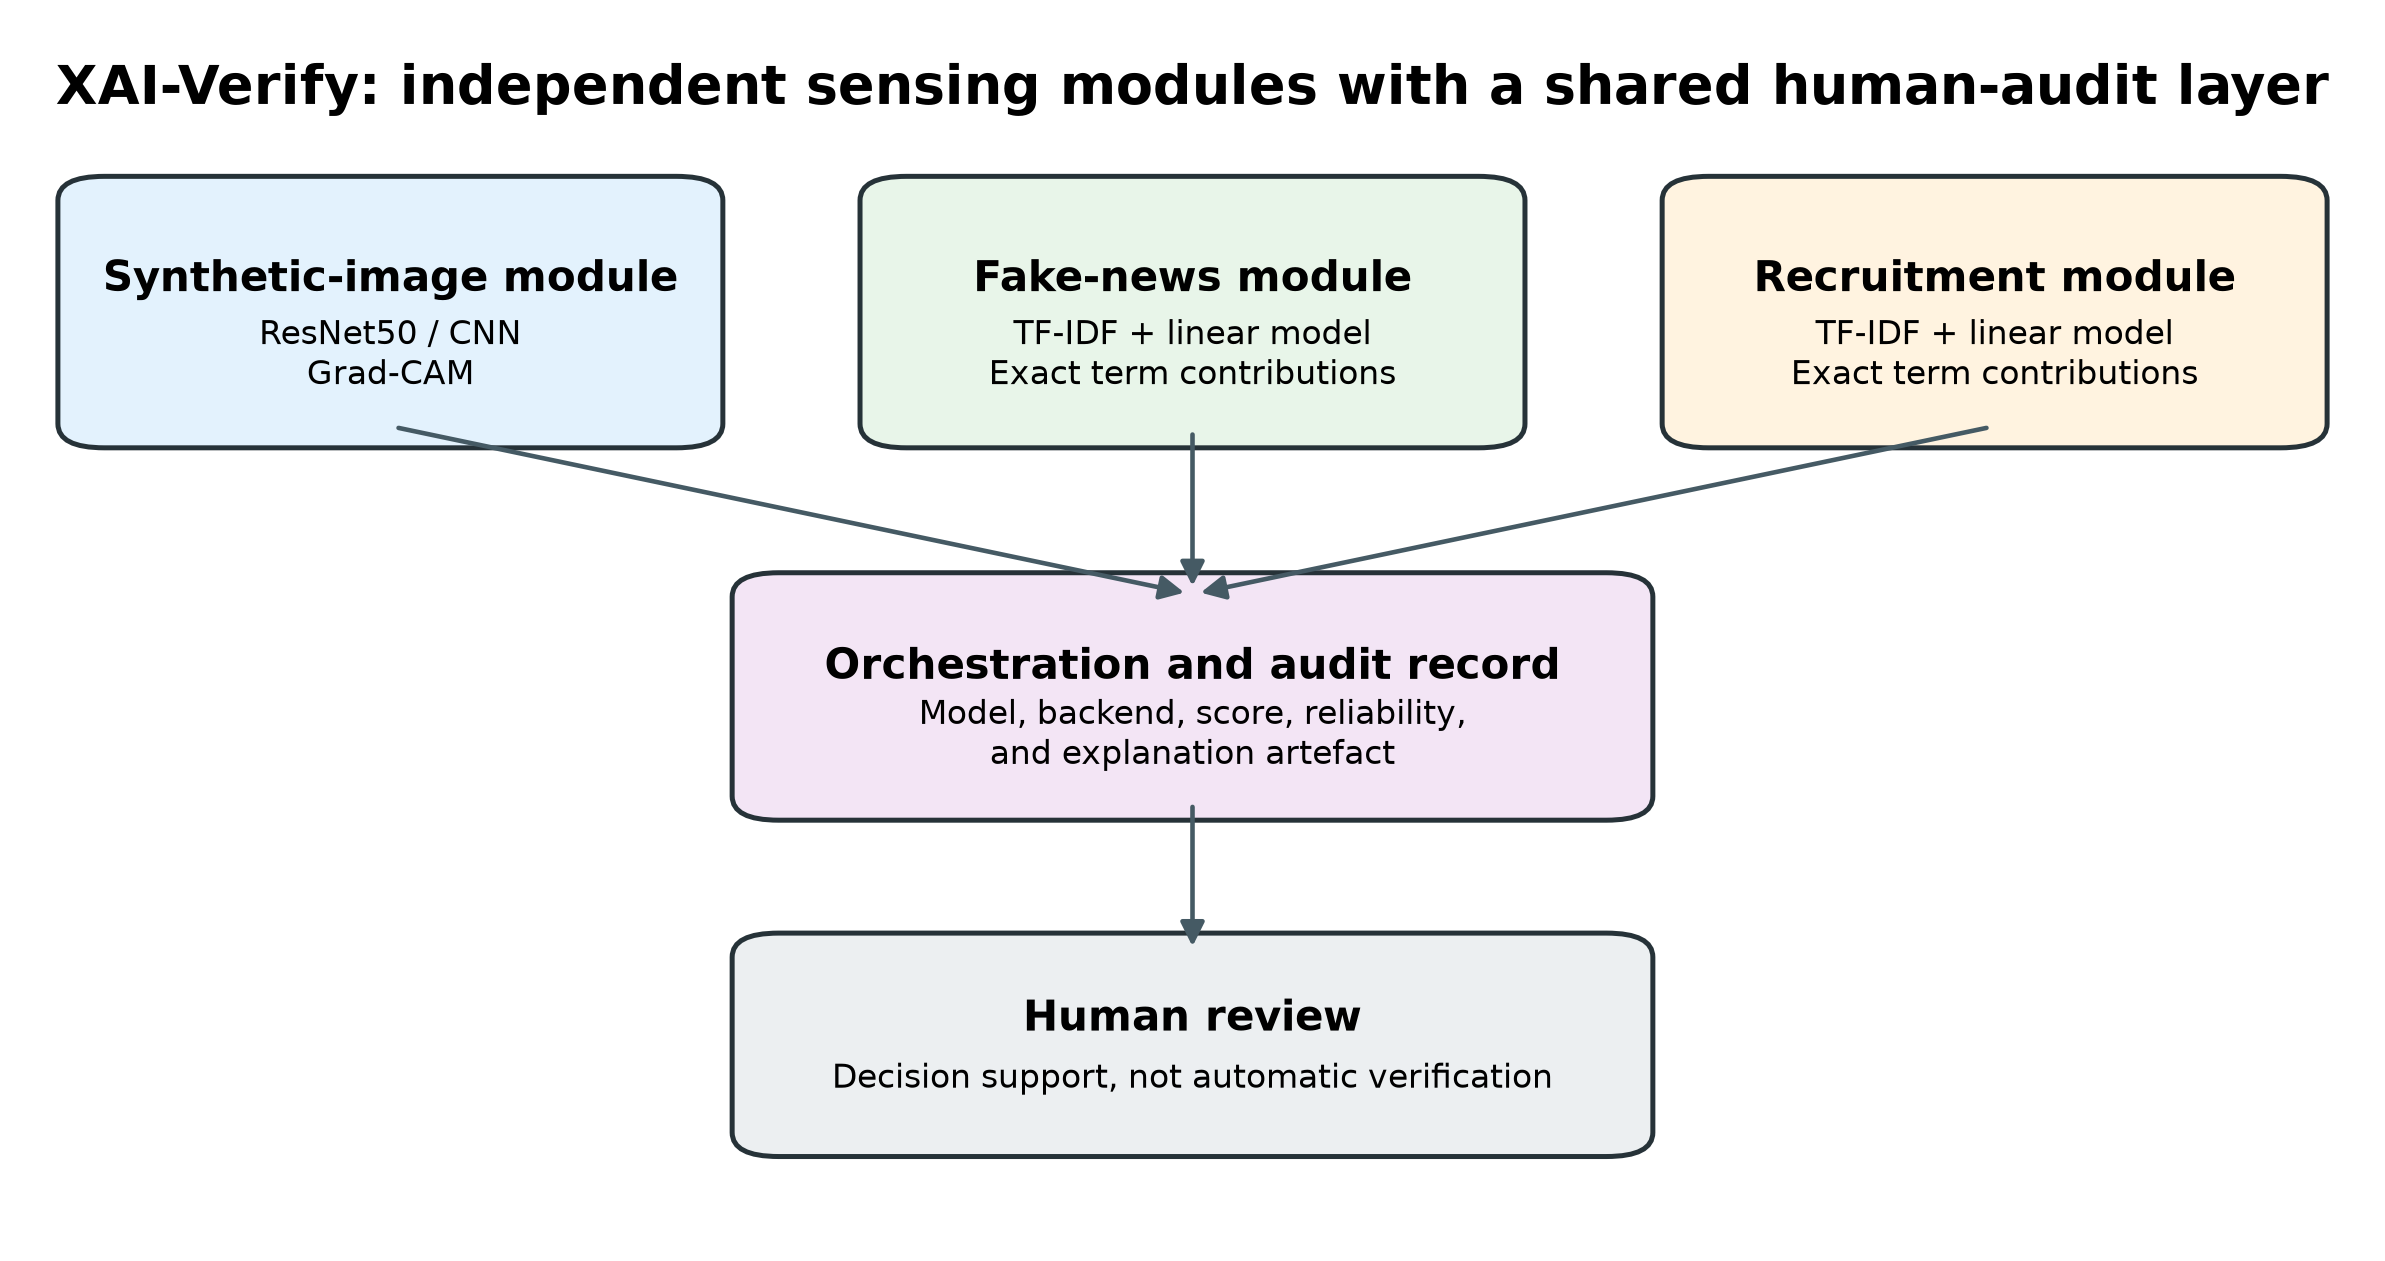
\includegraphics[width=\textwidth]{figs/system_architecture.png}
\caption{XAI-Verify system architecture. Three task-specific sensing modules produce predictions
and model-derived explanations. A shared orchestration layer records the model, backend, score,
reliability flag, and explanation for human review; outputs are not combined into a cross-task
vote.}\label{fig:architecture}
\caption*{\textit{Image description:} Three boxes for synthetic-image, fake-news, and recruitment
analysis feed an orchestration and audit-record box, which then feeds a human-review box.}
\end{figure}

\subsection{Image classifiers}
\textbf{Subset runs.} Four classifiers are trained under identical conditions on 5{,}000 random real and 5{,}000 random fake training images: ResNet50, EfficientNetB0 and MobileNetV2 \cite{he2016resnet,tan2019efficientnet,sandler2018mobilenetv2}, initialised from ImageNet weights, and a small four-block CNN (0.42M parameters) trained from scratch. A head of dropout (0.35), a 128-unit ReLU layer, dropout (0.25) and a sigmoid output gives the probability that an image is fake. Training has two stages: the backbone is frozen for four epochs (Adam, learning rate $10^{-3}$), then the last 40 backbone layers are unfrozen, with BatchNorm layers kept frozen, for two epochs at $10^{-5}$. We use early stopping and learning-rate reduction on validation loss and mild augmentation (horizontal flip, rotation $\pm4\%$, zoom 8\%, contrast 10\%). Validation and test use 3{,}000 random images per class from their own splits. An ablation on EfficientNetB0 removes fine-tuning or augmentation.

\textbf{Full-data run.} To use all 100{,}000 training images on CPU hardware, we keep the ImageNet ResNet50 backbone \emph{frozen}, extract its 2048-dimensional pooled features once for every image, and train classification heads on the cached features: logistic regression and an MLP (512 and 128 hidden units, dropout 0.4 and 0.3, early stopping on validation loss). Features are standardised with training-set statistics. The backbone is therefore not fine-tuned in this run. The trained pipeline is assembled into a single deployable model whose output matches the training pipeline to within $2\times10^{-4}$.

\subsection{Text classifiers}
Fake-news and recruitment texts are encoded with TF-IDF (word uni- and bigrams, sublinear term frequency, English stop words removed) and classified with L2-regularised logistic regression or a linear SVM, both with class weighting. For fake news we train on each corpus and test on all three. For recruitment, the decision threshold is chosen on the validation split only. The rule baseline uses payment, fee, and urgency phrases; a posting is flagged when any rule fires. We also evaluate a random forest and report 5-fold cross-validated F$_1$ on the training portion.

\subsection{Explanations}
\textbf{Grad-CAM.} For the image models we compute the gradient of the fake probability with respect to the last convolutional feature map, average it spatially to obtain channel weights, and form the rectified weighted sum of channels \cite{selvaraju2017gradcam}. Our implementation re-runs the saved model's preprocessing and head, and we verified that it reproduces the model's own prediction to within $6\times10^{-7}$ for ResNet50 and EfficientNetB0 models. \textbf{Word contributions.} For a linear model the decision score is the intercept plus the sum of weight$\times$TF-IDF value over terms, so each term's contribution is exact; this equals what SHAP's linear explainer reports up to a constant baseline \cite{lundberg2017shap}, and unlike LIME \cite{ribeiro2016lime} it requires no sampling. \textbf{Attention measure.} Faces in the main dataset are aligned crops, so the face lies near the centre. For each test image we measure the fraction of Grad-CAM mass inside the central $50\%\times50\%$ window, which covers 25\% of the image; a value of 0.25 means uniform attention. This is a coarse proxy (the feature map is $7\times7$) and not a face segmentation.

\subsection{Evaluation protocol}
We report accuracy, precision, recall, F$_1$ and ROC-AUC; for the imbalanced recruitment task we add PR-AUC. The positive class is ``fake'' or ``scam''. Confidence intervals are binomial (accuracy on the 20{,}000-image test set) or bootstrap (1{,}000 resamples). With 6{,}000 test images the 95\% interval on an accuracy near 0.85--0.90 is about $\pm0.8$--0.9 points. Models are compared on the same images with exact two-sided McNemar tests on paired correctness. \emph{Cross-domain} tests apply a trained model, without any retraining or threshold change, to a different dataset. For fake news we additionally train on pooled corpora and leave one corpus out; for recruitment we use repeated random splits and grouped cross-validation by employer (company profile), to separate generalisation to new employers from memorisation of known ones.

\section{Experimental Setup}
All experiments ran on a laptop with four CPU cores and 8~GB of RAM, without a GPU, using TensorFlow 2.21 and scikit-learn 1.9. Seeds are fixed. Each image network was trained once; the classifier heads of the training-source experiment are trained with three seeds, the recruitment experiments use five splits or folds, and the text classifiers are deterministic. No transformer text models were trained.

\section{Results}
\subsection{Image classifiers trained on 10{,}000 images}
All image models were evaluated on one common sample of 6{,}000 test images (3{,}000 per class), so that they can be compared directly (Table~\ref{tab:img}). Among the models trained on 10{,}000 images, the fine-tuned ResNet50 is the strongest (90.5\% accuracy, 95\% CI 89.7--91.2, AUC 0.971), ahead of EfficientNetB0 (84.7\%) and MobileNetV2 (83.5\%), which are close to each other. The small CNN trained from scratch reaches only 59.5\%, which shows how much the pre-trained features contribute at this data size. Exact McNemar tests on the paired predictions show that ResNet50 is significantly better than EfficientNetB0 and MobileNetV2 ($p<10^{-32}$), and that the difference between EfficientNetB0 and MobileNetV2 is marginal ($p=0.024$, not significant after correcting for the ten pairwise comparisons). The ablation (Table~\ref{tab:abl}) was run earlier on a different random sample of 6{,}000 test images, on which the full EfficientNetB0 scored 83.9\% instead of 84.7\%; the one-point difference is within the sampling error of about $\pm0.9$ points. It shows that fine-tuning adds about three accuracy points. Augmentation did \emph{not} help: removing it raised accuracy from 83.9\% to 86.1\%. A plausible reason is the short schedule (six epochs on 10{,}000 images); we did not test longer schedules, so this should not be read as a general conclusion.

\begin{table}[h]
\centering
\caption{Image classifiers on a common sample of 6{,}000 held-out test images (3{,}000 per class). The first row uses all 100{,}000 training images with a frozen backbone (Section~\ref{sec:full}); the others are fine-tuned on 10{,}000 images.}\label{tab:img}
\small
\begin{tabular}{lrrrrrr}
\toprule
Model & Params & Acc. [95\% CI] & Prec. & Rec. & F$_1$ & AUC \\
\midrule
ResNet50 + MLP head (frozen) & -- & \textbf{0.954} [0.949, 0.959] & 0.957 & 0.951 & \textbf{0.954} & \textbf{0.991} \\
ResNet50 (fine-tuned) & 23.9M & 0.905 [0.897, 0.912] & 0.926 & 0.881 & 0.903 & 0.971 \\
EfficientNetB0 (fine-tuned) & 4.2M & 0.847 [0.838, 0.856] & 0.857 & 0.833 & 0.845 & 0.931 \\
MobileNetV2 (fine-tuned) & 2.4M & 0.835 [0.826, 0.844] & 0.816 & 0.865 & 0.840 & 0.918 \\
Small CNN (scratch) & 0.4M & 0.595 [0.583, 0.606] & 0.575 & 0.726 & 0.642 & 0.638 \\
\bottomrule
\end{tabular}
\end{table}

\begin{table}[h]
\centering
\caption{EfficientNetB0 ablation on an earlier 6{,}000-image sample, distinct from the common
re-evaluation sample in Table~\ref{tab:img}; single training runs.}\label{tab:abl}
\begin{tabular}{lrrr}
\toprule
Variant & Acc. & F$_1$ & AUC \\
\midrule
Full (fine-tuning + augmentation) & 0.839 & 0.835 & 0.923 \\
No fine-tuning & 0.809 & 0.805 & 0.894 \\
No augmentation & 0.861 & 0.863 & 0.938 \\
\bottomrule
\end{tabular}
\end{table}

\subsection{Training on all 100{,}000 images}\label{sec:full}
Table~\ref{tab:full} shows the effect of using all 100{,}000 training images with a frozen ResNet50 backbone. A logistic-regression head reaches 90.0\% accuracy on the full 20{,}000-image test split, close to the 90.5\% obtained when the fine-tuned ResNet50 trained on 10\% of the data is re-evaluated on the common 6{,}000-image sample. Because the test samples differ, this is descriptive rather than a paired comparison. The non-linear MLP head reaches 95.4\% accuracy (95\% CI $\pm$0.3), F$_1$ 0.954 and AUC 0.990 on all 20{,}000 test images, so the gain comes from the combination of more data and a non-linear head. On a 6{,}000-image random subset of the test split the MLP's bootstrap intervals are 94.9--95.9\% (accuracy) and 0.990--0.993 (AUC), consistent with the full-test result. Validation accuracy was 94.8\% (MLP) and 89.9\% (logistic regression).

\begin{table}[h]
\centering
\caption{Frozen ResNet50 features, heads trained on all 100{,}000 training images; test on all 20{,}000 test images.}\label{tab:full}
\begin{tabular}{lrrrrr}
\toprule
Head & Acc. (95\% CI) & Prec. & Rec. & F$_1$ & AUC \\
\midrule
Logistic regression & 0.900 ($\pm$0.004) & 0.895 & 0.908 & 0.901 & 0.965 \\
MLP & \textbf{0.954} ($\pm$0.003) & 0.954 & 0.953 & 0.954 & 0.990 \\
\bottomrule
\end{tabular}
\end{table}

\subsection{Cross-domain image tests}\label{sec:cross}
Table~\ref{tab:cross} applies every image model, unchanged, to the two other image sets. All five perform at chance on balanced CIFAKE (48.6--50.0\% accuracy) and below the 56.4\% majority-class baseline on the local set (40.6--43.8\% accuracy); AUC is 0.35--0.48, indicating no useful ranking and, in several cases, slightly inverted scores. Four of the five models label almost every image as real (recall 0--4\% for the ``fake'' class). The failure is the same for models trained on 10{,}000 or 100{,}000 images, fine-tuned or frozen, and for three different architectures. These sets differ from the training data in several ways at once (content, resolution, generator, collection process), so the failure cannot be attributed to the generator alone; it does show that in-domain accuracy describes the training distribution and not detection of synthetic images in general.

\begin{table}[h]
\centering
\caption{Cross-domain tests without retraining: accuracy / AUC on the 6{,}000-image
training-domain test sample, CIFAKE (3{,}000 images), and the local independently collected set
(999 images).}\label{tab:cross}
\small
\begin{tabular}{lccc}
\toprule
Model & Same dataset & CIFAKE & Local set \\
\midrule
ResNet50 + MLP head (frozen, 100k) & 0.954 / 0.991 & 0.499 / 0.395 & 0.438 / 0.441 \\
ResNet50 (fine-tuned, 10k) & 0.905 / 0.971 & 0.498 / 0.419 & 0.431 / 0.401 \\
EfficientNetB0 (10k) & 0.847 / 0.931 & 0.499 / 0.419 & 0.429 / 0.417 \\
MobileNetV2 (10k) & 0.835 / 0.918 & 0.500 / 0.447 & 0.435 / 0.458 \\
Small CNN (scratch, 10k) & 0.595 / 0.638 & 0.486 / 0.484 & 0.406 / 0.353 \\
\bottomrule
\end{tabular}
\end{table}

\subsection{Mixed training sources}\label{sec:mixed}
To test whether adding a second generator repairs cross-domain failure, we hold the ImageNet ResNet50 backbone frozen, extract 2048-dimensional features once, and train the same MLP head under four data regimes (three seeds each): faces only (100{,}000 training images), CIFAKE only (9{,}000), all faces plus CIFAKE (109{,}000), and a balanced mix (9{,}000 faces subsampled plus 9{,}000 CIFAKE, 18{,}000 total). We evaluate on the held-out face test set (20{,}000 images), the CIFAKE test set (3{,}000) and a local collection of 999 images that never appears in training.

Table~\ref{tab:mixed} summarises accuracy and AUC (mean $\pm$ standard deviation over seeds where applicable). Training on faces alone yields strong in-domain performance (95.8\% $\pm$ 0.4) but chance-level CIFAKE accuracy (49.9\%). CIFAKE-only training inverts this pattern (93.4\% on CIFAKE, 48.0\% on faces) and gives the best local result (58.5\% $\pm$ 0.5), only modestly above the local set's 56.4\% majority-class baseline. Combining both sources in full raises CIFAKE accuracy to 92.9\% with essentially unchanged face-test accuracy (96.0\% $\pm$ 0.3), but local accuracy stays near 42\%. The balanced mix trades some face-test accuracy (88.4\%) for similar CIFAKE and local scores. Mixing generators therefore transfers performance between the two \emph{benchmark} image domains we control, but it does not close the gap on the independently collected local set, which differs in content and provenance in ways our protocol does not isolate.

\begin{table}[h]
\centering
\caption{Training-source ablation: frozen ResNet50 features, MLP head, mean $\pm$ std over three seeds (accuracy / AUC).}\label{tab:mixed}
\scriptsize
\resizebox{\textwidth}{!}{%
\begin{tabular}{lccc}
\toprule
Training data ($n$) & Face test (20k) & CIFAKE test (3k) & Local unseen (999) \\
\midrule
Faces only (100{,}000) & 0.958 $\pm$ 0.004 / 0.992 $\pm$ 0.001 & 0.499 / 0.407 & 0.435 / 0.431 \\
CIFAKE only (9{,}000) & 0.480 $\pm$ 0.009 / 0.430 $\pm$ 0.006 & 0.934 $\pm$ 0.004 / 0.983 $\pm$ 0.001 & 0.585 $\pm$ 0.005 / 0.592 $\pm$ 0.006 \\
Faces + CIFAKE, all faces (109{,}000) & 0.960 $\pm$ 0.003 / 0.992 $\pm$ 0.001 & 0.929 $\pm$ 0.001 / 0.981 $\pm$ 0.001 & 0.423 $\pm$ 0.007 / 0.411 $\pm$ 0.019 \\
Faces + CIFAKE, balanced (18{,}000) & 0.884 $\pm$ 0.006 / 0.955 $\pm$ 0.003 & 0.934 $\pm$ 0.002 / 0.982 $\pm$ 0.001 & 0.479 $\pm$ 0.012 / 0.477 $\pm$ 0.011 \\
\bottomrule
\end{tabular}
}
\end{table}

\subsection{Where the image model looks}
We computed the central-window attention share for 400 test images (200 per class) for the deployed model (Table~\ref{tab:attn}). The mean share is 0.367 (median 0.350), or 1.47 times a uniform spread: attention is moderately concentrated toward the centre, where the face lies, but about 63\% of the Grad-CAM mass still falls outside the central window. Shares are similar for real (0.394) and fake (0.340) images and for correctly (0.365) and incorrectly (0.397) classified images, so the measure does not separate right predictions from wrong ones; only 20 of the 400 images were misclassified, so the latter comparison is noisy. Figure~\ref{fig:gc} shows eight randomly chosen test images: in several of them the heat is on the eyes and forehead, but in others the strongest regions lie at the image corners, on clothing or on a hand, so we cannot say from this evidence that the model relies on facial features alone. The fine-tuned ResNet50 trained on 10{,}000 images behaved differently: on 500 test images its central share was 0.161 (0.65 times uniform; 0.124 for real and 0.199 for fake images), that is, more of its attention fell on the periphery than on the centre. All of these measures are coarse. We did not test whether the highlighted regions correspond to generation artefacts, and the cross-domain failures of Section~\ref{sec:cross} show that where a model looks within its training domain does not guarantee that it works elsewhere.

\begin{table}[h]
\centering
\caption{Share of Grad-CAM mass in the central $50\%\times50\%$ window (uniform attention = 0.25), deployed model, 200 test images per class.}\label{tab:attn}
\begin{tabular}{lrrr}
\toprule
Images & $n$ & Mean share & Ratio to uniform \\
\midrule
All & 400 & 0.367 & 1.47 \\
Real & 200 & 0.394 & 1.58 \\
Fake & 200 & 0.340 & 1.36 \\
Correctly classified & 380 & 0.365 & 1.46 \\
Misclassified & 20 & 0.397 & 1.59 \\
\bottomrule
\end{tabular}
\end{table}

\begin{figure}[h]
\centering
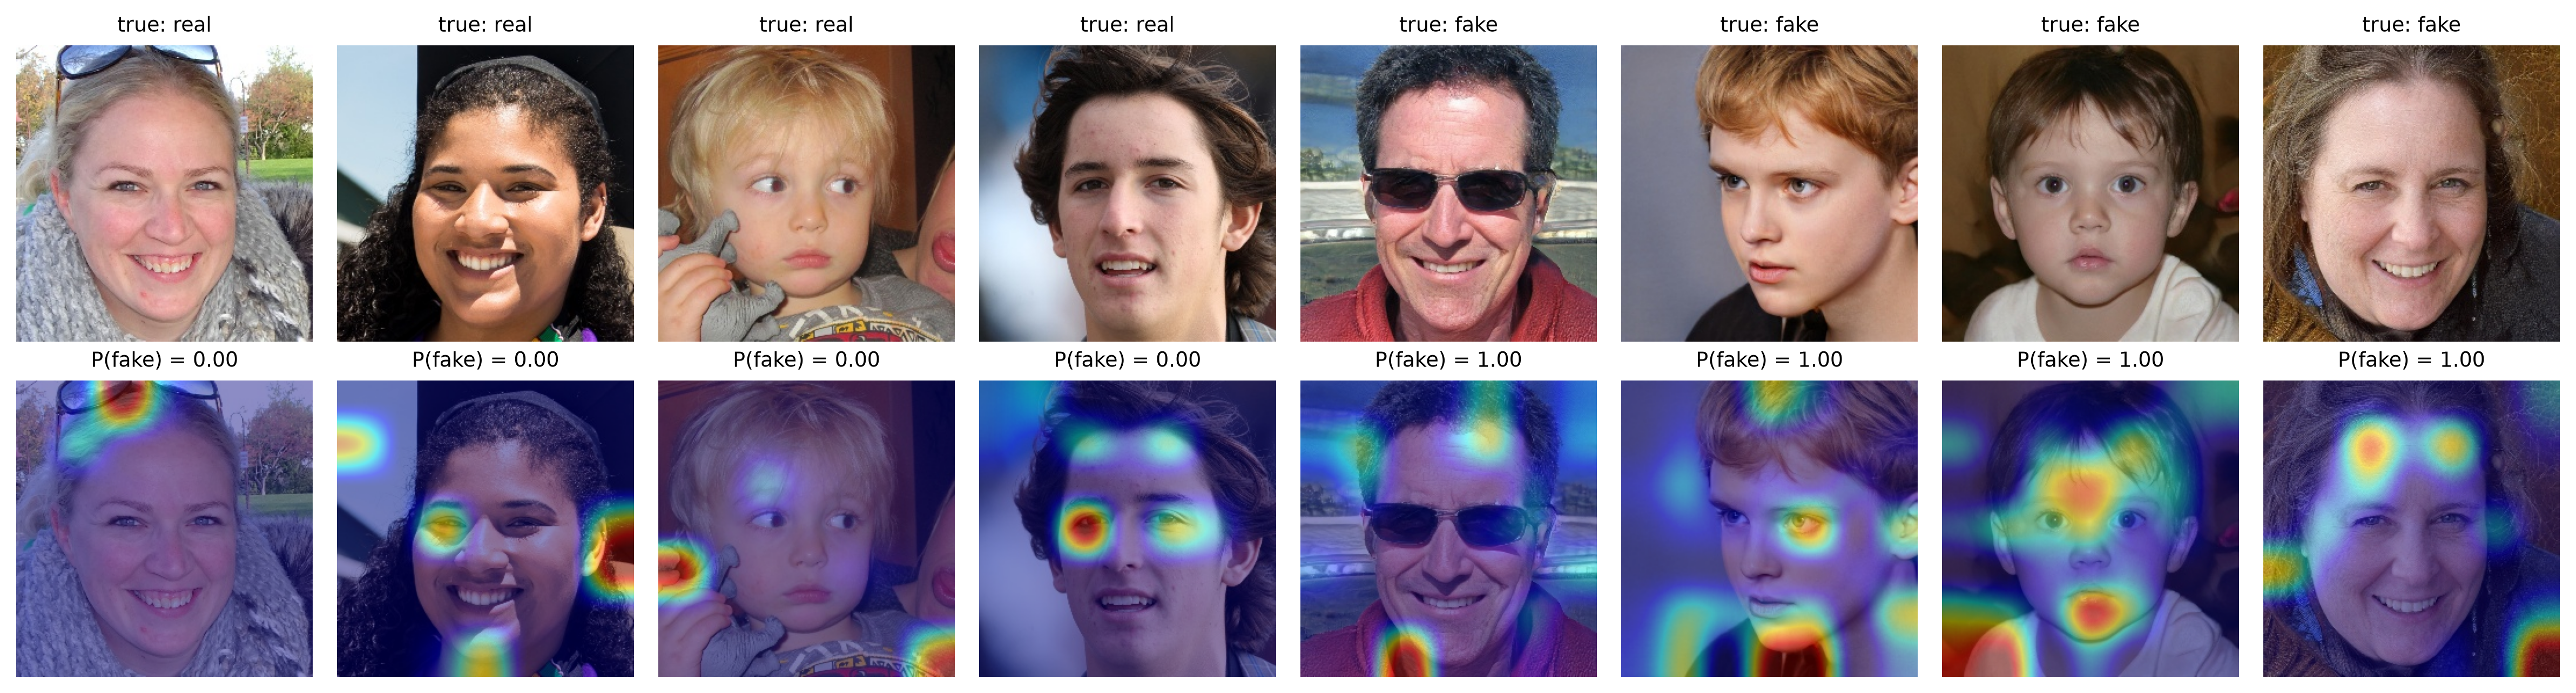
\includegraphics[width=\textwidth]{figs/gradcam_examples.png}
\caption{Grad-CAM of the deployed model on eight randomly chosen test images (fixed seed, not hand-picked): top row the images, bottom row the overlays with the predicted probability of ``fake''. All eight are classified correctly, with probabilities near 0 or 1.}\label{fig:gc}
\caption*{\textit{Image description:} Eight real or synthetic face crops appear above their
colour-coded Grad-CAM overlays. Warm regions indicate image areas with greater influence on the
model's synthetic-image score; attention varies between central facial regions and peripheral
background or clothing.}
\end{figure}

\subsection{Fake news: in-domain accuracy does not transfer}
Table~\ref{tab:news} (logistic regression; the linear SVM is within 0.5 points everywhere) shows the central result. In-domain accuracy is high (98.4\% on ISOT, 95.7\% on WELFake) but drops to 82.2\% when the ISOT model is tested on WELFake, and both article-trained models are at or below chance in accuracy on LIAR (44.7--48.4\%). Their F$_1$ scores are higher because the predictions are strongly skewed toward the positive class. A model trained on LIAR itself reaches 60.4\% accuracy, in line with the difficulty of that benchmark. The WELFake$\rightarrow$ISOT result (98.8\%) should not be read as generalisation, because WELFake merges sources of the same kind as ISOT and the corpora probably overlap.

The ISOT-trained model weights explain the gap. Terms most associated with \emph{real} news
include \texttt{said}, weekday names (\texttt{wednesday}, \texttt{tuesday},
\texttt{thursday}), \texttt{spokesman}, \texttt{reporters}, and \texttt{percent}; terms most
associated with \emph{fake} news include \texttt{video}, \texttt{watch}, \texttt{breaking},
\texttt{just}, \texttt{read}, and \texttt{mr}. These are cues of journalistic style and web
formatting, not evidence of truthfulness, and they are largely absent from one-sentence claims.

\begin{table}[h]
\centering
\caption{Fake-news logistic regression: accuracy / F$_1$ / AUC; rows are the training set and columns the test set. Diagonal entries are in-domain.}\label{tab:news}
\small
\begin{tabular}{lccc}
\toprule
Train $\backslash$ Test & ISOT & WELFake & LIAR \\
\midrule
ISOT & \textbf{.984} / .982 / .999 & .822 / .827 / .911 & .484 / .547 / .540 \\
WELFake & .988 / .986 / .999 & \textbf{.957} / .952 / .992 & .447 / .582 / .526 \\
LIAR & .592 / .586 / .637 & .581 / .566 / .619 & \textbf{.604} / .549 / .642 \\
\bottomrule
\end{tabular}
\end{table}

\textbf{Does pooling more sources help?} We also trained on pooled corpora (Table~\ref{tab:pool}). Training on all three corpora gives 99.1\% on ISOT and 96.3\% on WELFake, but still only 59.9\% on LIAR, the same as training on LIAR alone (60.4\%). In leave-one-corpus-out tests, the model trained on the other two corpora reaches 82.0\% on WELFake and 45.8\% on LIAR, no better than single-corpus models. (The 98.9\% obtained on a held-out ISOT is again inflated by WELFake's overlap with ISOT.) Adding more article-level data therefore does not teach the models to judge claims. The LIAR intervals are wider (about $\pm2.6$ points) because the LIAR test set has only 1{,}283 statements.

\begin{table}[h]
\centering
\caption{Fake news with pooled training (logistic regression): accuracy [95\% bootstrap CI].}\label{tab:pool}
\small
\begin{tabular}{lccc}
\toprule
Setting & ISOT & WELFake & LIAR \\
\midrule
Single corpus, in-domain & 0.984 [0.981, 0.987] & 0.957 [0.953, 0.961] & 0.604 [0.578, 0.629] \\
Pooled (all three corpora) & 0.991 [0.988, 0.993] & 0.963 [0.959, 0.967] & 0.599 [0.571, 0.624] \\
Leave this corpus out (train on the other two) & 0.989 [0.986, 0.991] & 0.820 [0.812, 0.827] & 0.458 [0.432, 0.485] \\
\bottomrule
\end{tabular}
\end{table}

\subsection{Recruitment-scam detection}
Table~\ref{tab:job} shows that the rule baseline performs at chance (ROC-AUC 0.506, F$_1$ 0.06): its payment and fee patterns, written for a different style of scam, almost never match EMSCAD's English postings. On the fixed split, the trained linear models reach F$_1$ of 0.80--0.81 (5-fold cross-validated F$_1$ 0.83--0.85), and the random forest is weaker (0.73). Dropping the structured fields (logo, questions, salary) leaves F$_1$ unchanged at 0.80, so the text-only model, which is the one a web form can supply, is the deployed one. The fixed test split contains only 107 fraudulent postings, so its F$_1$ has a wide bootstrap interval (0.80, 95\% CI 0.73--0.86; recall 0.72, CI 0.63--0.81).

\textbf{Split variance and employer memorisation.} Two further protocols (Table~\ref{tab:jobprot}) change the picture. Over five random stratified splits the text-only model reaches F$_1$ $0.849\pm0.033$, so the fixed split was on the low side. But when entire employers are held out, using grouped 5-fold cross-validation by company profile (4{,}767 distinct employer groups), F$_1$ falls to $0.600\pm0.158$ (precision $0.67\pm0.25$, recall $0.60\pm0.15$). Postings from the same employer are therefore easier to classify than those from new employers, consistent with the company-specific terms among the top-weighted features (for example \texttt{accion}); terms pointing toward scam otherwise include \texttt{data entry}, \texttt{earn}, \texttt{money} and \texttt{clerical}. The deployed model should be expected to perform closer to the grouped estimate on postings from employers it has not seen.

\begin{table}[h]
\centering
\caption{Text-only logistic regression on EMSCAD under different evaluation protocols (mean $\pm$ standard deviation).}\label{tab:jobprot}
\small
\begin{tabular}{lrrrr}
\toprule
Protocol & Prec. & Rec. & F$_1$ & PR-AUC \\
\midrule
Fixed split (deployed model), bootstrap CI for F$_1$ & 0.895 & 0.720 & 0.798 [0.733, 0.861] & 0.837 \\
Five random stratified splits & $0.907\pm0.061$ & $0.800\pm0.048$ & $0.849\pm0.033$ & $0.902\pm0.018$ \\
Grouped by employer, 5-fold CV & $0.671\pm0.250$ & $0.601\pm0.148$ & $0.600\pm0.158$ & $0.694\pm0.128$ \\
\bottomrule
\end{tabular}
\end{table}

\begin{table}[h]
\centering
\caption{Recruitment-scam detection on EMSCAD (2{,}382 test postings, 107 scams; scam is the positive class).}\label{tab:job}
\begin{tabular}{lrrrrr}
\toprule
Model & Prec. & Rec. & F$_1$ & PR-AUC & ROC-AUC \\
\midrule
Rule-based baseline & 0.056 & 0.065 & 0.060 & 0.046 & 0.506 \\
TF-IDF + logistic regression & 0.868 & 0.738 & 0.798 & 0.866 & 0.987 \\
TF-IDF + linear SVM & 0.907 & 0.729 & \textbf{0.808} & \textbf{0.875} & 0.987 \\
Random forest & 0.779 & 0.692 & 0.733 & 0.816 & 0.975 \\
Logistic regression, text only (deployed) & 0.895 & 0.720 & 0.798 & 0.837 & 0.963 \\
\bottomrule
\end{tabular}
\end{table}

\subsection{Implementation}
The detectors are served by a web application. Explanations are computed from the deployed models;
heuristic explanation placeholders were excluded from the evaluated system. Inputs shorter than 30
words receive a reliability warning because the fake-news model is near chance on short claims.

\section{Discussion}
Across all three modules, in-domain scores overstated what the detectors do elsewhere. All five image models, including the one that scores 95.4\% on its own distribution, are at chance on two other image sets; the fake-news classifiers lose about 16 points on a second news corpus and fall to chance on claim-level data; the recruitment classifier drops from F$_1$ 0.85 to 0.60 when it must classify postings from employers it has not seen; and the rule-based recruitment method is at chance on a standard corpus. Where we could inspect the models (fake news and recruitment), the highest-weight features were dataset or style cues rather than evidence of deception, which is the likely mechanism of the failures. For practitioners, the implication is that a detector's accuracy should be reported together with a test on data from a different source (or, for text about organisations, on unseen organisations), and that explanations should be inspected for what they reveal about the features used, not only shown to end users.

More data and a non-linear head raised in-domain image accuracy substantially (Table~\ref{tab:full}) but did not change cross-domain behaviour, and pooling article-level corpora did not help on claims (Table~\ref{tab:pool}). The mixed-source experiment (Section~\ref{sec:mixed}) shows a systems-level lesson: enlarging the training \emph{system boundary} to include a second labelled generator improves transfer between those generators, yet a third, independently collected test stream still behaves like an open environment. From a cybernetic viewpoint, the detector's feedback signal (labels) is tied to each corpus's generative and editorial process; mixing two controlled sources does not automatically produce a sensor that generalises to an unmodelled third. We also removed source tags from ISOT and WELFake, and we recommend doing the same, because otherwise these corpora can be solved by a single string.

\section{Limitations and Threats to Validity}
\label{sec:limits}
\begin{itemize}
\item \textbf{Frozen backbone in the full-data run.} The 95.4\% model does not fine-tune ResNet50; fine-tuning on all 100{,}000 images would probably score higher and may behave differently across domains. The fine-tuned models used 10\% of the training data.
\item \textbf{Single runs of the image networks.} Each fine-tuned image network was trained once, so differences of one or two points between configurations (for example, the augmentation result) may be within seed variation; McNemar tests account only for test-set sampling, not for training variability.
\item \textbf{No transformer text models.} The text modules use TF-IDF with linear models; we make no claim about transformer behaviour across datasets.
\item \textbf{Cross-domain test sets differ in many ways.} The two other image sets differ from the training data in content, resolution, generator and collection process at once, so we cannot attribute the failure to any single factor; the local independently collected set is small and of mixed origin.
\item \textbf{Small positive class.} The recruitment fixed test split has 107 scams, and the grouped cross-validation has high variance across folds (F$_1$ standard deviation 0.16); EMSCAD also contains company-specific cues.
\item \textbf{Dataset effects.} The face dataset is aligned crops from one source; WELFake probably overlaps ISOT; LIAR is binarised from six labels.
\item \textbf{Coarse attention measure.} The central window is a proxy for the face, and the $7\times7$ Grad-CAM map is coarse.
\end{itemize}

\section{Conclusion}
A single explainable pipeline for deepfake images, fake news and recruitment scams is feasible on modest hardware, but evaluation protocol matters more than model choice. A ResNet50-feature classifier trained on 100{,}000 images reaches 95.4\% on its own test set, and all five image models we trained fail on other image sets; fake-news accuracy collapses across corpora and on claim-level data, and pooling article corpora does not help; a learned recruitment model clearly beats hand-written rules but loses much of its accuracy on unseen employers. Computing explanations from the models themselves exposed what they rely on. Future work should fine-tune the full network on all data with repeated runs, add transformer baselines, test more generators and domains, and measure explanation faithfulness with deletion, insertion, and sanity-check protocols \cite{adebayo2018sanity,petsiuk2018rise}.

\section*{Acknowledgments}
No acknowledgments are included in the anonymous manuscript. Any identifying acknowledgments will
be added after peer review.

\section*{Author contributions}
The authors' CRediT roles are supplied on the separate title page to preserve double-anonymous review.

\section*{Funding}
\textbf{[AUTHORS TO CONFIRM: ``This research received no specific grant from any funding agency in
the public, commercial, or not-for-profit sectors.'' OR INSERT THE EXACT FUNDER AND GRANT NUMBER.]}

\section*{Disclosure statement}
\textbf{[AUTHORS TO CONFIRM: ``The authors report no competing interests.'' OR INSERT THE
APPROPRIATE DISCLOSURE.]}

\section*{Ethics statement}
This study used publicly released benchmark datasets and did not recruit participants or intervene
with human subjects. The system is a research prototype and its outputs should not be used as the
sole basis for legal, employment, or content-moderation decisions.

\section*{Declaration of generative AI use}
Generative AI tools were used to assist software development and manuscript language, formatting,
and reference organisation. The authors reviewed the generated material, verified the reported
experiments and cited sources, and take full responsibility for the content of the manuscript.

\section*{Data and code availability}
The face, CIFAKE, ISOT, WELFake, LIAR, and EMSCAD datasets are publicly available from the sources
cited in the Materials section. Cleaning, splitting, training, and evaluation scripts, together
with derived result tables, will be deposited at \textbf{[INSERT PUBLIC REPOSITORY URL AND
PERSISTENT IDENTIFIER OR ANONYMOUS REVIEW LINK]}.

\bibliographystyle{unsrtnat}
\bibliography{references}

\end{document}
